%------------------
% General Settings
%------------------
\def \docTitle      {Application Note}
\def \docSubTitle   {Measurement of the four Stokes parameters}
\def \productNumber {}
\def \productName   {}
\def \docAuthor     {LK-Instruments}
\def \docRevision   {Rev. 001}
\def \docSubject    {\docAuthor \docTitle \docSubTitle}
\def \docKeywords   {\docAuthor, \productName, \productNumber, SMC2242, SMC4242, M101}

\documentclass[a4paper, final, 12pt, oneside]{scrartcl}

%----------
% Packages
%----------
\usepackage{etex}
\reserveinserts{30}
\usepackage[utf8]{inputenc}
%\usepackage[latin1]{inputenc} % erlaubt Umlaute in der tex-Datei

\usepackage{slantsc}
\usepackage[urw-garamond]{mathdesign}
\usepackage{garamondx}
\usepackage[T1]{fontenc}

\usepackage[english]{babel}              % For the hyphenations in different languages
\usepackage[intlimits]{amsmath}          % math symbols
\usepackage{braket}                      % Dirac braket notation
\usepackage{graphicx}                    % include pictures
\usepackage{color}
\usepackage[shell]{gnuplottex}           % gnuplot in latex
\usepackage{pstricks}                    % post script tricks
\usepackage{listings}                    % enter programming code
\usepackage{fancyhdr}                    % make quite nice header/footer
%\usepackage[version=3]{mhchem}           % chemistry stuff
\usepackage{relsize}
\usepackage{afterpage}
\usepackage{gensymb}
\usepackage{textcomp}
\usepackage{multicol}
%\usepackage{subfig}
\usepackage{lipsum}
\usepackage{multirow,booktabs,colortbl,tabularx}
\usepackage{caption}
\usepackage{subcaption}


\usepackage{pgfplots}
\usepackage{tikz}                        % beautiful plots
\pgfplotsset{compat = newest}
\usepackage{units}                       % easy to use number-unit-package
\usepackage[section]{placeins}           % Float barrier for sections.


\usepackage{listings}					% erlaubt Quellcode mit Zeilenumbruechen
\usepackage{float} % l�dt das Paket zum erzwingen der Grafikposition

%----------------
% PDF properties
%----------------
\usepackage[
  pdftitle={\docAuthor~\docSubTitle~\docTitle}
 ,pdfsubject={\docSubject}
 ,pdfauthor={\docAuthor}
 ,pdfkeywords={\docKeywords}
 ,pdfcreator={\docAuthor}
 ,pdfstartview=Fit                       % startseite ganz anzeigen
 ,pdfborder={0 0 0}                      % links ohne umrandungen
 ,pdfdisplaydoctitle=true                % pdftitle statt dateinamen anzeigen
 ,pdfcenterwindow=true                   % position pdf in center of the screen
 ,setpagesize=true
]{hyperref}

%-------------------
% Header und Footer
%-------------------
\fancyhf{}        % clear all header/footer
\renewcommand{\headrulewidth}{0pt}
%\renewcommand{\sectionmark}[1]{\markboth{#1}{}}
%\renewcommand{\subsectionmark}[1]{\markright{#1}}
\fancyhead[RE,RO]{\productNumber}
\fancyfoot[LE,LO]{\docAuthor}
\fancyfoot[CE,CO]{\docRevision}
\fancyfoot[RE,RO]{\thepage}

\pagestyle{fancy}

% number equations with sections before equation-index
%\numberwithin{equation}{section}
%\numberwithin{table}{section}
%\numberwithin{figure}{section}

%---------------------
% My code definitions
%---------------------

\newtheorem{envdefinition}{Definition}[section]
\newtheorem{envsatz}{Satz}

% special numbers and letters
\renewcommand{\i}{\mathrm{i}}                  % complex i
\newcommand{\e}{\mathrm{e}}                    % Eulers number
\renewcommand{\phi}{\varphi}                   % nicer phi
\renewcommand{\epsilon}{\varepsilon}           % nicer epsilon
\renewcommand{\theta}{\vartheta}               % nicer theta
\renewcommand{\rho}{\varrho}                   % nicer rho
%\newcommand{\degree}{^{\circ}}                 % degree-circle

% vectors and matrices
\renewcommand{\vec}[1]{\boldsymbol{#1}}
\newcommand{\Vek}[3]{\left(\begin{array}{c}#1\\#2 
\ifthenelse{\equal{#3}{}}{}{\\#3}\end{array}\right)}

% integral and derivative stuff:
\renewcommand{\d}[1]{\;\mathrm{d}#1}           % integeration d
% total derivative
\newcommand{\td}[1]{\frac{\mathrm{d}}{\mathrm{d}#1}\,}
\newcommand{\pd}[1]{\partial_{#1}\,}             % partial derivative

% Braket notation
\renewcommand{\bra}{\Bra}
\renewcommand{\ket}{\Ket}
\renewcommand{\braket}{\Braket}
\renewcommand{\set}{\Set}

% plus-minus with braces
\newcommand{\PM}{\ensuremath{\substack{+\\[-0.25em]-}\,}}
\renewcommand{\pm}{\PM}
\newcommand{\pmp}{\ensuremath{\substack{\mathsmaller{(}+\mathsmaller{)}\\[-0.25em]-}\,}}
\newcommand{\pmm}{\ensuremath{\substack{+\\[-0.25em]\mathsmaller{(}-\mathsmaller{)}}\,}}

\setlength{\columnsep}{40.0pt}

%----------------------------------------------------------
% let the party start
%----------------------------------------------------------
\begin{document}
\setlength{\parindent}{0pt}
       
\begin{minipage}{\textwidth}
  \begin{minipage}[h]{0.125\textwidth}
      
\includegraphics[width=1\textwidth]{../general/logo_black.pdf}
  \end{minipage}
  \hfill
  \begin{minipage}[h]{0.8\textwidth}
      {\Huge \textbf{\textsf{\docTitle}}} \\
      {\Large \textbf{\textsf{\docSubTitle}}}
  \end{minipage}
\end{minipage}       
       
\vspace*{5pt}
\rule{\textwidth}{0.4pt}

This Application note describes how the Stepper Motor Controller SMC4242 can be used together with the Rotation Stage M101 to measure an arbitrary polarisation state.\\
The polarisation state of electromagnetic radiation can be expressed by the Stokes parameters ($S_0$, $S_1$, $S_2$ and $S_3$). To measure the four Stokes parameters of polarized light a setup like the one shown in figure~\ref{setup_stokes} can be used.
 The Stokes parameters can be obtained by performing the measurements listed in table~\ref{stokes_measurements}.

\begin{figure}[h]
\begin{center}
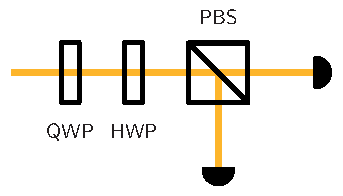
\includegraphics[width=8cm]{Grafiken/polarization_measurement.pdf}
\caption[Setup for measurement of the four Stokes parameters.]{Setup for measurement of the four Stokes parameters. It consists of a quarter waveplate (QWP), a half waveplate (HWP), a polarizing beam splitter (PBS) and two detectors.}
\label{setup_stokes}
\end{center}
\end{figure}

\begin{table}[H]
\centering
\begin{tabular}{c|c|c|c} 
Stokes parameter & QWP & HWP & detector signals \\ \hline
$S_0$ & $\unit[0]{{^\circ}}$ ($0$) & $\unit[0]{{^\circ}}$ ($0$) & add \\
$S_1$ & $\unit[0]{{^\circ}}$ ($0$) & $\unit[0]{{^\circ}}$ ($0$) & subtract \\
$S_2$ & $\unit[45]{{^\circ}}$ ($\frac{\pi}{4}$) & $\unit[22.5]{{^\circ}}$ ($\frac{\pi}{8}$) & subtract \\
$S_3$ & $\unit[45]{{^\circ}}$ ($\frac{\pi}{4}$) & $\unit[45]{{^\circ}}$ ($\frac{\pi}{4}$) & subtract \\
\end{tabular}
\caption[Measurement of the four Stokes parameters.]{Measurement of the four Stokes parameters ($S_0$, $S_1$, $S_2$ and $S_3$) using the setup shown in figure~\ref{setup_stokes}. The waveplates need to be set to the given angles with respect to the vertical axis and the electrical sum or difference of the detector signals needs to be taken.}
\label{stokes_measurements}
\end{table}

In order to facilitate the implementation we provide a sample program \\
\textsf{sample\_measureStokesParameter.py}\\
on our website \href{http://www.lk-instruments.com}{www.lk-instruments.com}. In this sample program it is assumed, that the quarter waveplate (QWP) is mounted on the Rotation Stage attached to channel 0 of the Stepper Motor Controller and that the Rotation Stage carrying the half waveplate (HWP) is connected to channel 1. In addition it is assumed, that the $\unit[0]{{^\circ}}$ position corresponds to a situation where the fast axis of a waveplate is vertical.


\end{document}
